\section{BPMN Extension}\label{ch:bpmnx}

% maybe cite braun2015behind

The extensibility mechanism of the \ac{BPMN} allows to extend standard process elements with additional attributes, while maintaining conformity with the BPMN core~\cite[p.\,44]{bpmnspec}.
%Extensions are specified through an external definitions file and can be included into a BPMN process model by reference.
The BPMN extension developed in the present work is revealed in this section. First, an overview is provided (\autoref{bpmnx:overview}), then a more detailed documentation of the functionality and usage is provided.
%- structure of this section: overview (initial understanding of the extended notation and the semantics), usage documentation(, detailed execution semantics?)

\subsection{Overview}\label{bpmnx:overview}
This section introduces a novel BPMN extension for incorporating event subscription semantics in business process models.
The extension develops around the addition of subscription-related attributes to the BPMN \textit{Message} type. Based on the additional information, subscription and un-subscription for message events is handled automatically by an especially adapted process engine.
The added attributes are \textit{EventQuery}, \textit{SubscriptionTime} and \textit{BufferPolicies}:
\textit{EventQuery} contains an arbitrary query string; \textit{SubscriptionTime} defines when the subscription should happen; \textit{BufferPolicies} is a complex type which influences the behavior of the related event buffers.
Only \textit{EventQuery} is a mandatory parameter, all others will fall back to default values if not provided.
An overview of all possible fields, values and their defaults is provided in \autoref{tab:bpmn-extension}.

% variables in the event query

The presented extension is to be used in connection with intermediate catch events, boundary events and receive tasks through their direct or indirect association with the message element.
Additionally, the \textit{Event Subscription Task}, an extension of the \textit{Task} is introduced. It adds a single additional attribute \textit{messageId} to \textit{Task} and can thereby be used to manually trigger the subscription for the associated message element as part of the execution flow of a process.
%- for the others, the subscription and unsub from the event source is managed implicitly by the underlying infrastructure
By the use of the \textit{SubscriptionTime} variable, the event subscription can be issued before the process flow reaches the event element and listens for the message. %bpmn event element is listening.
Any messages that arrive before the event element is active are temporarily stored and will be delivered to the catch event or receive task once it is active.
These storages as referred to as \textit{Event~Buffers}. By default, they store the latest message they receive, though the behavior can be adjusted using the \textit{BufferPolicies}.

%- it is required that the infrastructure is prepared to execute extended processes accordingly, ref chapter
% though, theoretically, every message can be extended with the attributes, the subscription is only managed for the elements...

\begin{table}
	\myfloatalign
	\begin{tabularx}{\textwidth}{p{0.3\linewidth} p{0.515\linewidth} c}
		\toprule
		\tableheadline{Attribute Name} & \tableheadline{Value Options (\underline{default})} & \tableheadline{Req.} \\ 
		\midrule
		EventQuery & any query string & y \\
		SubscriptionTime & process-deployment,\newline process-instantiation,\newline manual, \underline{element reached} & n \\
		BufferPolicies & Complex Type (see below) & n \\
		
		\midrule
		\tableheadline{bufferPolicies}  \\
		\midrule
		
		LifespanPolicy & string in ISO time-span format OR '\underline{infinite}' & n \\
		ConsumptionPolicy & \underline{reuse}, bounded-reuse(n), consume & n \\
		SizePolicy & positive integer, \underline{1}, 0 means infinite & n \\
		OrderPolicy & \underline{FIFO}, LIFO & n \\
		
		\bottomrule
	\end{tabularx}
	\caption[Available attributes of \textit{SubscriptionDefinition} in the BPMN extension for flexible event subscription]{Available attributes of \textit{SubscriptionDefinition} in the BPMN extension for flexible event subscription}  
	\label{tab:bpmn-extension}
\end{table}

\subsection{Documentation}

Through the BPMN extension, subscription-related information can be added to the Message element.
While other authors have chosen to add subscription information directly to the catch event \cite{Baumgrass2016,beyer2016unicorn}, the Message element has been chosen for several reasons: It is a good match semantically, subscription meta information about an event message has a close relation to the Message element itself; By extending the Message element, a single extension applies to the intermediate event, the boundary event and the receive task at the same time (the extension is specifically designed for the use with exactly these three elements); If a single Message shall be used in a process multiple times, the subscription information must only be provided once.
% receiveTask.messageRef; boundaryEvent.catchEvent.(message)eventDefinition.messageRef; intermediateCatchEvent.catchEvent.(message)eventDefinition.messageRef
%Each of the three elements references a BPMN \textit{Message}, the common denominator for communication within and across business processes.

By specification, the \textit{Message} element comprises an attribute \textit{name}, the name of the message, and \textit{itemRef}, the reference to a BPMN \textit{ItemDefinition} specifying the Message structure. Additionally, it inherits all attributes from the BPMN \textit{RootElement}~(see \cite{bpmnspec}\,p.\,93).
In the following, the required additional attributes will be explained one after the other. A complete list is available in \autoref{tab:bpmn-extension}. The goal is to retain a stand-alone model that contains all information necessary to execute the subscription to the event source.
All subscription information is incorporated in a model element \textit{subscriptionDefinition}, which is added to the \textit{extensionDefinitions} of the Message element.
The formal XSD-Schema is available in the appendix, \autoref{lst:xsd-flexsub}.

%\subsubsection{Introducing Event Buffers}
%Any event message that occurs before reaching the event element but after the time of subscription will be kept in a buffer by the system.
%In its simplest version, the buffer is of length 1, that means it stores exactly one message received from a CEP platform. It always stores the latest message. When a newer message arrives, the old one is replaced in the buffer.
%\autoref{ch:bpmnx:bufferpolicies} introduces a set of advanced buffer policies to adapt this behavior further.
%\todo[inline]{By default, there is no interference between the buffers of different messages, process instances or processes. Each buffer instance will contain the latest information as if it was the only buffer in the system. Performance improvements to avoid duplicate buffer content will be managed by the system without explicit action by the user. Section ... later introduces a shared, more complex usage scenario of the event buffers.}

\subsubsection*{Adding basic subscription information}\label{ch:bpmnx:basic}

For a subscribe operation, we consider the event~query, the platform address and optionally authorization information of the CEP~platform.
This extension assumes that only one event engine is in use, so that access information can be configured in a central configuration store for the current process execution environment and not redundantly for each message.
The event query instead needs to be specified for every message and is added to the model as an extension attribute \textit{eventQuery} of type \textit{string}, which should contain the full query as interpretable by the CEP platform.

Given this first fundamental part of the BPMN extension, it is possible to execute the subscription, thus addressing requirement R1. However, the time of subscription cannot be influenced.

\subsubsection*{The time of event subscription modeled in BPMN}\label{ch:bpmnx:subscriptiontimes}

This section specifically addresses the requirement \textit{R2}, aiming to provide a flexible event subscription time to be selected for each BPMN message when designing an event-driven process.
Two different means are to be offered to support all subscription times demanded by \textit{R1.1}: Firstly, the subscription can happen in the background. Alternatively, the subscription can be modeled explicitly as a flow-element in the process.
It is a task of the process design phase, to elaborate the correct time of subscription necessary for the use case.

The subscription will be executed automatically by the system based on the information given in the BPMN model. Further information on the exact execution flow is provided in \autoref{bpmnx:executionsemantics}.
As this means that the subscribe and unsubscribe operations themselves do not have to be explicitly modeled, shortcoming \textit{S2} is addressed.



\paragraph{Subscription time as part of the BPMN Message element\newline}
To provide the Process Designer with a simple but powerful tool to influence the time of event subscription, a field \textit{subscriptionTime} is added the BPMN message element. 
The field can take one of the following values: \textit{process-deployment}, \textit{process-instantiation}, \textit{manual}, \textit{element-reached}. The last option is the default option, intepreting the standard BPMN semantics.
Note that a \textit{subscriptionTime} set to \textit{element-reached} will remain without effect if an explicit subscription task for the same event was executed before the event is reached.

In motivating Example~1.1 (\autoref{ch:motivatingexamples}), it is necessary to issue the subscription to the Eurotunnel event as early as possible to make sure that data is available and the process execution is not delayed.
Using the BPMN extension, the use case can be implemented by defining the event query and the subscription time in the BPMN model as depicted in \autoref{lst:xml-message-onInst}.

\begin{lstlisting}[caption={XML representation of an extended BPMN Message element},label=lst:xml-message-onInst]
<bpmn:message id="sample-message" name="SampleMessage">
  <bpmn:extensionElements>
    <flexsub:subscriptionDefinition>
      <flexsub:eventQuery>SELECT delay, occurrenceTime, delayReason FROM eurotunnel</flexsub:eventQuery>
      <flexsub:subscriptionTime>process-deployment</flexsub:subscriptionTime>
    </flexsub:subscriptionDefinition>
  </bpmn:extensionElements>
</bpmn:message>
\end{lstlisting}


\paragraph{The event subscription task\newline}
As an alternative to specifying the subscription time using the extension field \textit{SubscriptionTime}, an extension to the BPMN \textit{Task} type is proposed. 
The extended task is used to execute the subscription explicitly as part of the process flow.
A field \textit{messageId} is added to the service task to establish a reference between the activity and the message definition.
As introduced in section~\autoref{ch:bpmnx:basic}, the extended BPMN Message definition contains the information necessary to issue the subscription to an event source.
Once the Explicit Subscription Task is activated, the subscription for the referenced message is issued. 

Modeling the event subscription in an explicit task can be necessary when the subscription depends on the result of another activity. In that case, the subscription cannot be issued on process instantiation, because the necessary information is not yet available. Instead, an early subscription can be implemented using the extended service task.
Apart from this particular use case, the explicit subscription task enables the Process Designer to place the subscription flexibly in the process flow and give her full control over the time of subscription.

If both tools, the extension field \textit{SubscriptionTime} and the explicit subscription task, are used for a single BPMN message, the earlier subscription of the two will be executed, the second subscription will have no effect.
That means for example if the \textit{SubscriptionTime} is set to \textit{event reached} and an explicit subscription task is inserted before the event element, then the subscription will be executed at the time the explicit subscription task is active.
If \textit{SubscriptionTime} is set to \textit{Process Deployment}, then the subscription will happen at that time and the explicit subscription task will remain without effect.
In case neither of the two is used, the system falls back to the BPMN default and executes the subscription when the event element is reached.

\subsubsection{Using Process Variables in Event Queries}\label{ch:bpmnx:variables-in-queries}

% also see bpmn2 spec 10.3 pp. 233ff.

As shown in motivating example~2 (\autoref{ch:motivatingexamples}), it can be the case that the current values of process data must be dynamically used in an event query.
Therefore, the name of the dataObject should be part of the event query. At the time of subscription, the mentioned variable is dynamically replaced by its current value.
The exact notation for including process variables in event queries may vary depending on the employed query language so that it does not interfere with any existing notation schemes.
For the use with the Esper EPL, the following is suggested: The exact name of the variable has to be surrounded by curly brackets and preceded by a \textit{\#} character: \textit{\#\{VARIABLENAME\}}.
This notation is inspired by the usage of substitution parameters in SQL queries that are embedded in Esper EPL. They take a similar form, though using a \$ sign\footnote{see~\textit{5.13.1. Joining SQL Query Results}, \url{http://www.espertech.com/esper/release-5.3.0/esper-reference/html/epl_clauses.html}, accessed 2017-08-13}.

The use of dynamic process variable values introduces an additional complexity: Depending on the time of event subscription, the value of the process variable might not yet be available.
Variables are replaced by their runtime values at the time of event subscription and an execution error is invoked if the required information is not available, causing the process instance to be stopped.

\subsubsection{Advanced Buffer Parameters}\label{ch:bpmnx:bufferpolicies}
This section of the documentation addresses requirement \textit{R3}.

\paragraph{Lifespan of buffered events\newline}

The \textit{LifespanPolicy} allows to specify after which timespan elements in the buffer should be deleted. Timespans are defined using the ISO8601 notation for time intervals\footnote{see \textit{Date and time format - ISO 8601}, \url{https://www.iso.org/iso-8601-date-and-time-format.html}, accessed 2017-08-13}. 
The default value is \textit{infinite}.

Motivating Example~1.1 is implemented by setting the \textit{SubscriptionTime} to \textit{process-deployment}, which means that there can be an infinite time difference between the action of subscribing to the event source and the reaching of the event element in one of the instances.
In case events are not published in a longer time, for example due to technical fault at the event producer, the buffer will contain older events that might not be relevant anymore.
Using the \textit{LifespanPolicy}, the process designer can express, that events should be deleted from the buffer after a certain period of time and thus avoid outdated information. The buffer is maintained automatically by the system.
That of course comes at the price that the process has to remain in waiting state until a new event message arrives.

\paragraph{Consumption Behavior}

So far, the event buffers can be used isolated from each other. There is no interference between buffer instances and events are not removed from the buffer after retrieval.
While for most use-cases this behavior is sufficient, more detailed control over the buffer can be desirable when a given message is accessed multiple times. More precisely, if an event element is activated multiple times or multiple elements reference the same \textit{Message} element, then the consumption behavior must be clear.
Not always is it wanted, that events remain in the buffer after retrieval.
An additional parameter \textit{ConsumptionPolicy} is introduced which can take the values \textit{consume}, \textit{reuse}(default) and \textit{bounded reuse(n)}.
While \textit{reuse} denotes the behavior that is already known, \textit{bounded reuse(n)} will allow an element to be retrieved exactly \textit{n} times. \textit{n} has to be replaced by an integer value greater 0.
The option \textit{Consume} will remove an element from the buffer immediately after it has been retrieved for the first time, it is therefor equivalent to \textit{Bounded Reuse(1)}.

Given the possibility to \textit{consume} from an event buffer, more complex scenarios can be designed.
Let us consider the flight booking process shown in \autoref{fig:example-flightbooking}: A request for flight booking offers is issued as a manual Event Subscription Task instantiating an Event Buffer. The referenced message with the identifier \textit{FlightOffer} is modeled with a \textit{manual} \textit{SubscriptionTime} and the \textit{ConsumptionPolicy} set to \textit{consume}.
The receipt of flight offers is modeled as an Intermediate Catch Event referencing the same message. After the receipt of the first offer, the offer is deleted from the buffer and the sequence flow proceeds to the activity \textit{Evaluate Offer}.
The buffer can receive flight offers during the evaluation of the first offer.
When the evaluation is finished, either another offer is considered from the event buffer or decision-making is closed and the best offer is selected from all offers that where considered so far.
Using the consuming buffer, the same buffer can be accessed multiple times in a single process without using the same event every time.

\begin{figure}[]
	\myfloatalign
	{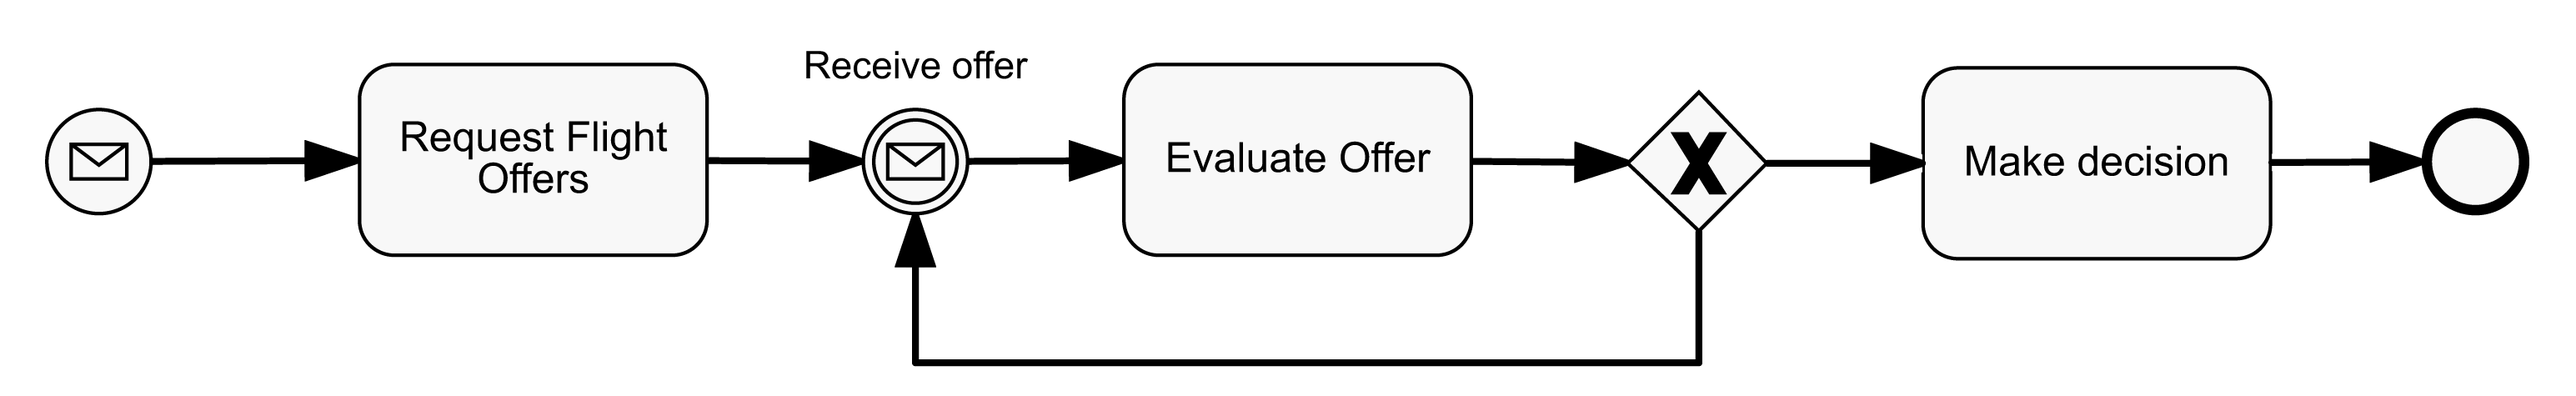
\includegraphics[width=1\linewidth]{chapters/concept/bpmnx/FlightBooking.png}}
	\caption{Simplified model of a flight Booking process using a consuming buffer}\label{fig:example-flightbooking}
\end{figure}

In that regard, the scope of a buffer is defined as follows: If the subscription time is \textit{on-deployment}, a buffer ranges all instances of a given process. If it is set to \textit{on-instantiation}, the buffer only ranges the one instance of the process. A buffer shared across multiple process definition is assumed when the subscription time is set to \textit{manual} and the referenced message share the same message identifier and subscription information across all process definitions in scope.

A possible use case for a shared buffer is shown in \autoref{fig:example-complaints}. Within an organization, multiple processes might exist to handle complaints. The referenced message elements share the same event query, manual subscription time and the \textit{consume} policy across all these process definitions. \autoref{fig:example-complaints} shows how the events are retrieved from the shared buffer in \textit{obtain complaint} and then processed. In the course of the gateway it is either decided to process another complaint using the given process or to end the process execution.

\begin{figure}[]
	\myfloatalign
	{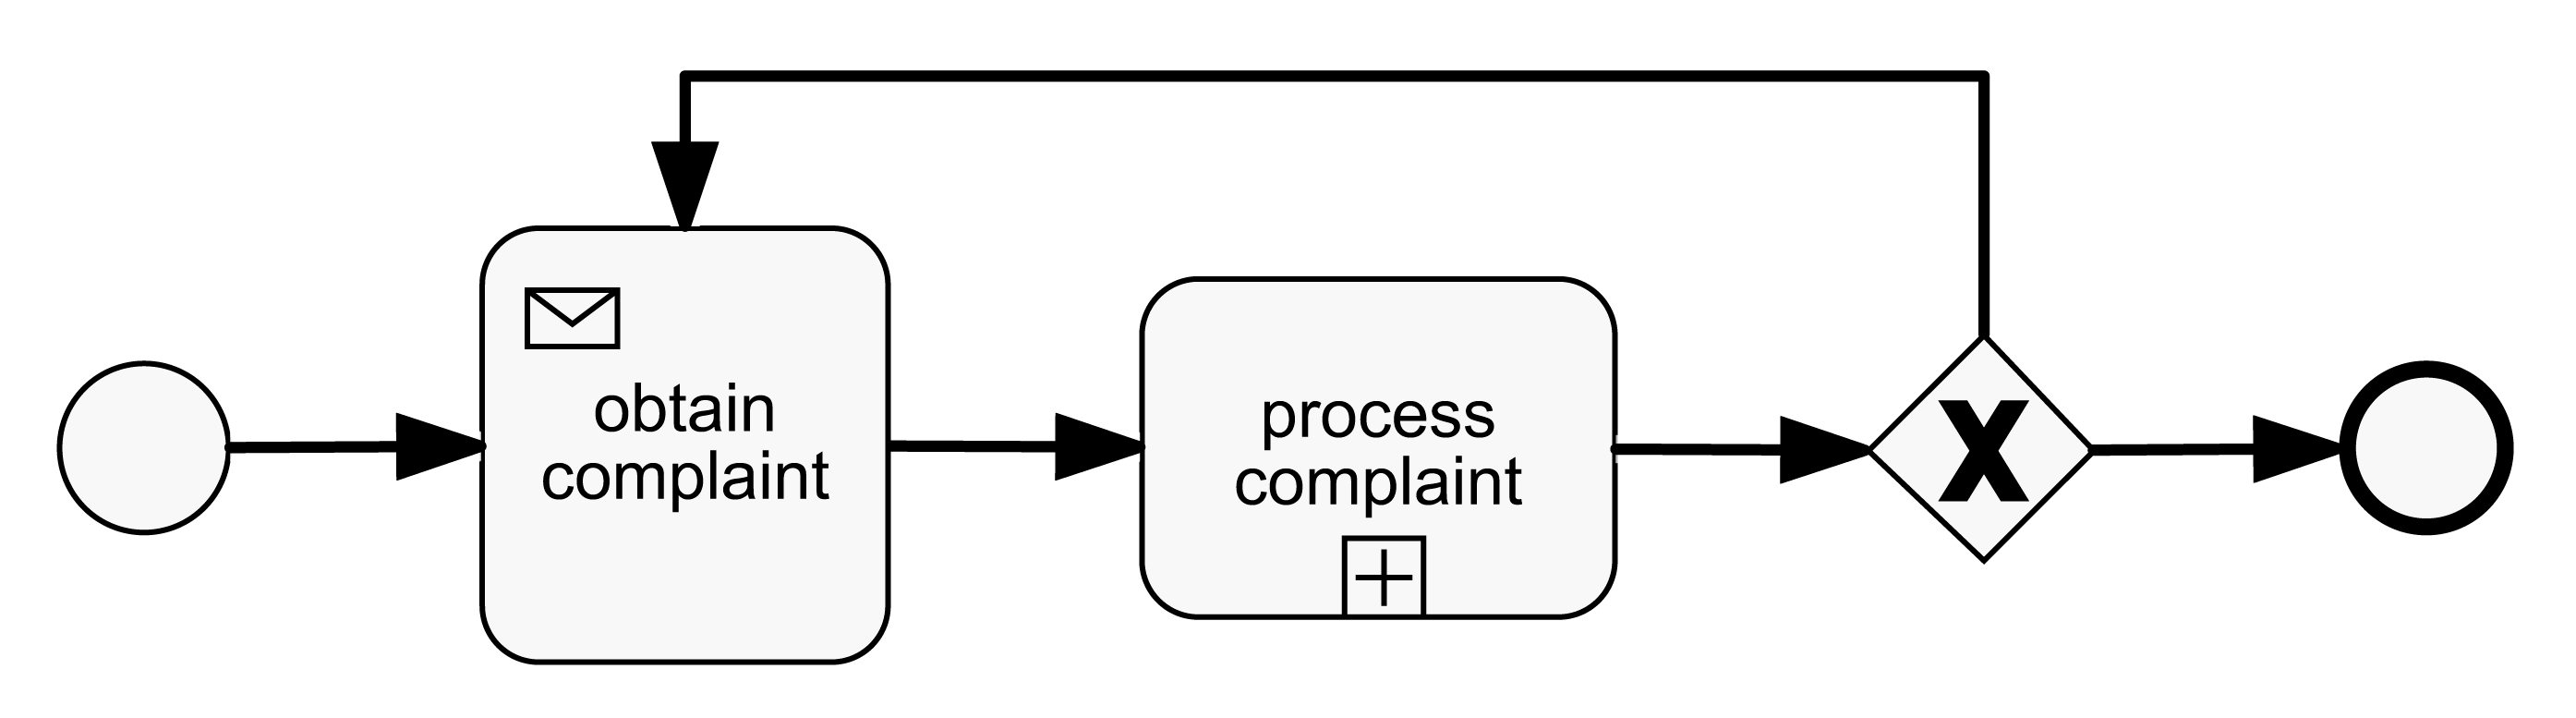
\includegraphics[width=1\linewidth]{chapters/concept/bpmnx/ComplaintProcessing.png}}
	\caption{Shared consuming buffer in a simplified model of a complaints handling process}\label{fig:example-complaints}
\end{figure}

\paragraph{Buffer Size and Order Policy}
Offering the option to consume from buffer instances that are reused within a process instance, across multiple instances of the same process or across multiple processes implies the need to additionally specify the number of elements that are stored in the buffer and the order of retrieval from the buffer.

The order policy can be either \textit{FIFO} (first in first out) or \textit{LIFO} (last in first out). Accordingly, the buffer either behaves like a queue (FIFO) or a stack (LIFO). The default value is \textit{FIFO}.
The size of the buffer is denoted as a positive integer value, whereas \textit{0} means that the buffer is of infinite size, the default behavior. If the buffer contains its maximum number of elements, the element that would be retrieved from the buffer last (considering the order policy) is removed from the buffer.

\subsection{Execution Semantics}\label{bpmnx:executionsemantics}

After the previous section has described the functionality and usage of the BPMN extension, the following section textually defines the additions necessary to the BPMN execution semantics to implement the subscription, the un-subscription and the interaction with the event buffer.
According to the specification, the purpose of the execution semantics is \textit{to describe a clear and precise understanding of the operation of the elements}.~\cite{bpmnspec},\,p.\,425\,ff.
While the execution semantics in BPMN must not be supported for a product to achieve \textit{Modeling Conformance}, they must be implemented to achieve \textit{Process Execution Conformance}.

\paragraph{Life cycle of event elements}
The semantics are described in accordance with the activity instance life cycle \cite[p.\,84]{weske:bpm-book}, which defines the states and transitions any activity instance traverses during process execution (\autoref{fig:activity-lifecycle}).
When a process is instantiated, also activities are initialized and enter the init state.
Once the execution activates the incoming flow of an activity, its state changes to \textit{ready} and can enter the \textit{running} state any time. If the activity execution completes without interruption, it traverses into \textit{terminated}, if the execution is interrupted through a boundary event, it ends in the \textit{canceled} state.
If an activity never enters the \textit{running} state because the process flow proceeded on a different branch, the activity is skipped.

Originally, this life cycle specifically relates to activity instances.
To specify the execution semantics of the presented extension, for example the time of subscription and un-subscription, a similar model is required for describing the life cycle of event elements.
For this purpose, the life cycle of an event is considered to consist of the same states and transitions as an activity.
Event elements can be canceled when they appear after an event-based gateway and another event following the same gateway occurs earlier.
If the trigger of the event fires, it enters \textit{terminated}. Equivalent to activities, event elements can be skipped if the process execution choses a different path.

\begin{figure}[]
	\myfloatalign
	{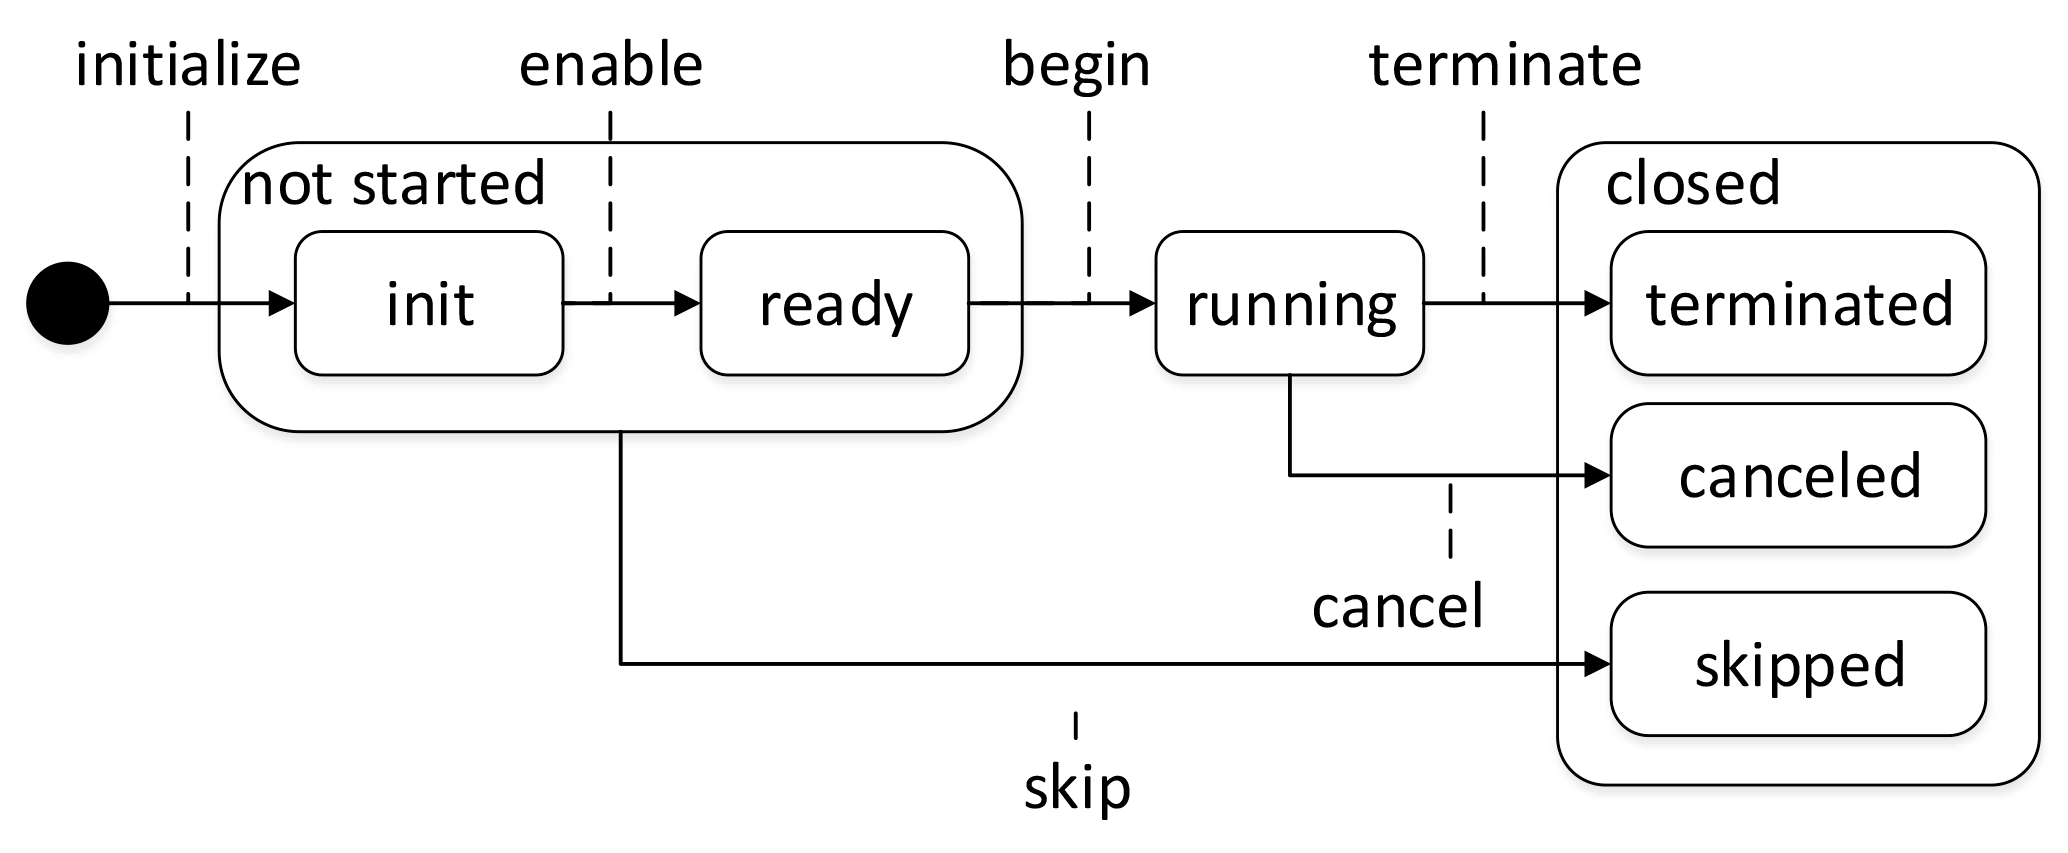
\includegraphics[width=1\linewidth]{chapters/concept/bpmnx/activity-lifecycle.png}}
	\caption{The activity instance life cycle}\label{fig:activity-lifecycle}
\end{figure}

\paragraph{Operational Semantics for subscription handling}
The subscription behavior of the existing BPMN elements intermediate message catch event (IMCE), boundary message catch event (BMCE) and receive task (RT) can be defined using the \textit{subscriptionDefinition} extension inside the associated Message element.
%For the purpose of enhancing their operational semantics for automatic subscription handling, either of the three is referred to as a \textit{receiving element}
Furthermore, the subscription can be modeled as a flow element using the \textit{Event Subscription Task}.
Each of these elements already has execution semantics defined by the BPMN specification, which are extended with additional operations for flexible event handling.
Due to the possibility to define the \textit{SubscriptionTime} independently from the event element or receive task, adopting the semantics for these four elements is not sufficient to implement all possible event subscription times.

Because the execution semantics are reliant on the subscription time specified in the message, the enhanced semantics are not described per element, but for each possible subscription time.
The required additions to the operational semantics of BPMN are as follows:

\begin{description}
	\item[SubscriptionTime \textit{element reached}:]
	IMCE/BMCE/RT: The subscription to the event source is issued on the \textit{begin} transition. The element remains in \textit{running} state until an event is consumed. The un-subscription from the event source is performed either on the \textit{terminate} or on the \textit{cancel} transition.
	
	\item[In every other case:] 
	IMCE/BMCE/RT: On the \textit{begin} transition, events are requested from the Event Buffer associated to the element.
	The element remains in \textit{running} state until the buffer delivers an event or the \textit{cancel}	transition takes place.
	When the \textit{cancel} or the \textit{terminate} transition is performed, the buffer is informed to stop delivering events.
	
	\item[SubscriptionTime \textit{process-deployment}:]
	The BPMN specification itself states that the \textit{deployment of Business Processes [is] out of scope} \cite[p.\,22]{bpmnspec}.
	However, there must be a certain operational semantic implied by the start of the listening process to Message Start Events.
	Therefore: An Event Buffer for the Message element is initialized at the end of the process deployment process. At the same time when the listening process to a Message Start Event begins.
	The Event Buffer is destroyed when the process gets un-deployed, the same time a Message Start Event stops listening.
	
	\item[SubscriptionTime \textit{process-instantiation}:] 
	The Event Buffer for the Message element is created when the Start Event that initializes the process instances creates a token on its outgoing Sequence Flows, that means after the start event has occurred.
	The Event Buffer is destroyed when the process instance terminates, more precisely, when all tokens of the process instance have reached an end node (a node without outgoing sequence flows).
	
	\item[Subscr. through explicit subscription task:]
	An Event buffer for the referenced Message is initialized when the Event Subscription Task performs the \textit{begin} transition.
	The deletion of the buffer follows the same rules as in \textit{Subscr. on process instantiation}
	
	\item[SubscriptionTime \textit{manual}:]
	The existence of an event buffer instance is assumed, hence no further operations are specified.
\end{description}



